\section{Discretization of the Mat\'ern SPDE}
\label{sec:discretization_matern}

In the following analysis we consider a 3D field
$\uni(\x)$, $\x\in\domain$ and show the discretized form for $\maternop^{-M}$.
We begin by showing the form for $M=1$, and then simply illustrate how the
operator can be applied iteratively for $M>1$.
We carry out the discretization on a structured, nonuniform, Arakawa C
grid \citep{arakawa_computational_1977}
according to the finite volume method - as is the general setting in the MITgcm.
We note that our development is similar to \citet{fuglstad_exploring_2015},
who show a differential operator for a 2D field on a uniform grid.

\cref{fig:mitgcm_grid} shows the general structure of the grid, and
defines the various grid cell distances used in the derivation.
We begin by integrating \cref{eq:spde_general},
\begin{linenomath*}\begin{equation}
    \begin{aligned}
        \int_{\domain} \delta(\x)\,\uni(\x)\, d\x -
        \int_{\domain} \nabla\cdot K(\x)\nabla\,\uni(\x)\,d\x
        &=
        \int_{\domain} \W(\x)\defdet^{-1/2} \, d\x \\
        \sum_{\ijk}\int_{\cell_\ijk} \delta(\x)\,\uni(\x)\, d\x -
        \sum_{\ijk}\int_{\cell_\ijk} \nabla\cdot K(\x)\nabla\,\uni(\x)\,d\x
        &=
        \sum_{\ijk}\int_{\cell_\ijk} \W(\x)\defdet^{-1/2} \, d\x \, ,
    \end{aligned}
    \label{eq:spde_integral}
\end{equation}\end{linenomath*}
where in second line we distribute the integral across each grid cell
$\cell_\ijk\subset\domain$ and $\ijk$ indicates indices in longitude, latitude,
and depth, respectively.

\begin{figure}
    \centering
    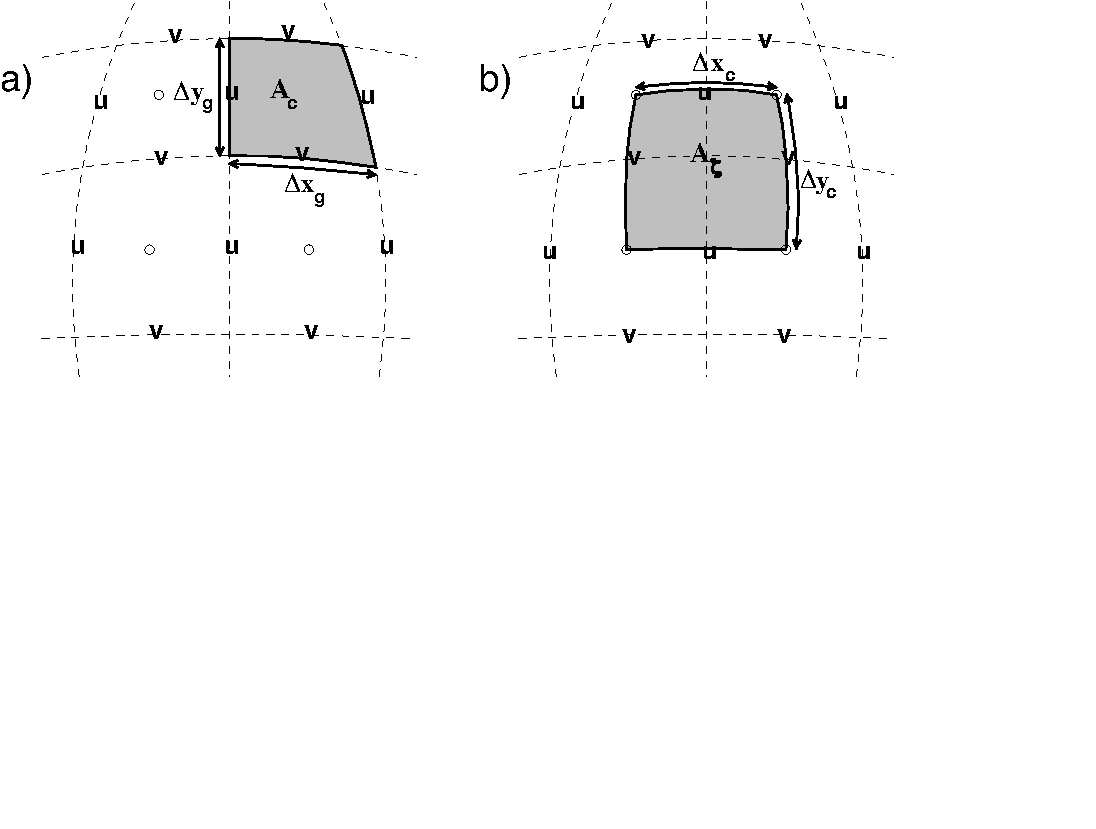
\includegraphics[width=.6\textwidth]{../figures/hgrid-abcd.pdf}
    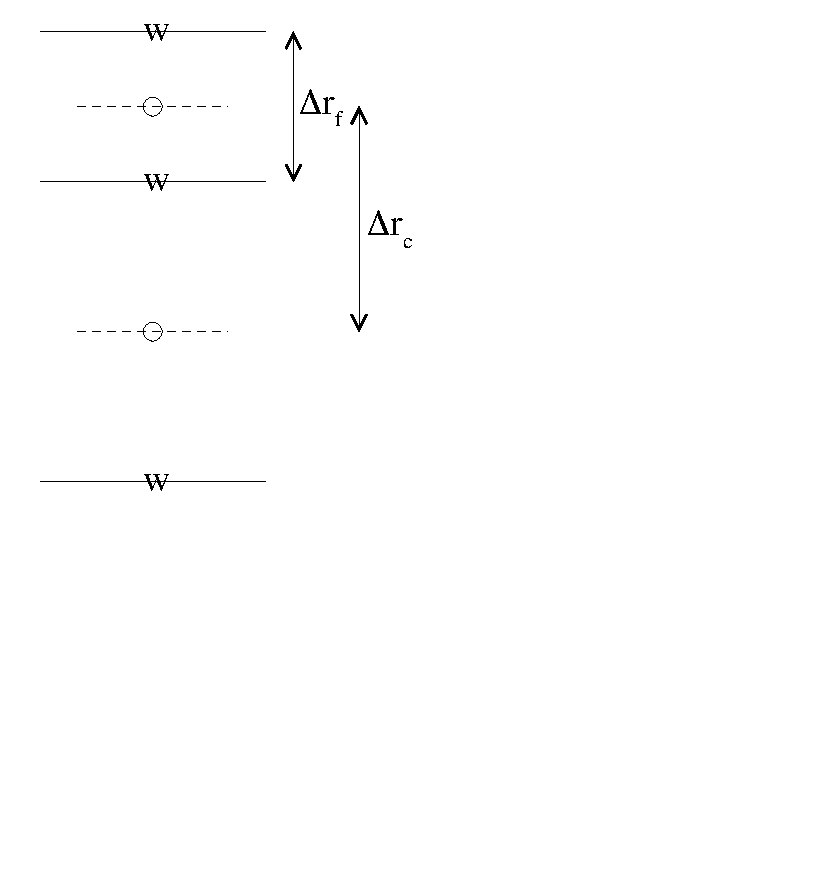
\includegraphics[width=.2\textwidth]{../figures/vgrid-accur-center.pdf}
    \caption{The structured finite volume grid used in the MITgcm. The
        left two figures show the horizontal grid, viewed from above. The right
        figure shows the vertical grid. In each figure, u, v, and w mark the
        location where velocities exist on the grid cell interfaces. The open
        circles denote the tracer location at the grid cell center,
        where fields like temperature and salinity are located. Figures are from
    \citet{campin_mitgcmmitgcm_2021}.}
    \label{fig:mitgcm_grid}
\end{figure}

Starting with the first term,
\begin{linenomath*}\begin{equation*}
    \begin{aligned}
        \delta_\ijk &\coloneqq \dfrac{1}{\vol_\ijk}\int_{\cell_\ijk}\delta(\x)\,d\x
        \\
                   &=
                   \dfrac{\deltah}{\vol_\ijk}\int_{\cell_\ijk}\dfrac{1}{\defdetd}\,d\x
    \end{aligned}
\end{equation*}\end{linenomath*}
so that
\begin{linenomath*}\begin{equation*}
    \int_{\cell_\ijk} \delta(\x)\,\uni(\x)\, d\x =
    \deltah\dfrac{\vol_\ijk}{\defdetd}\uni_\ijk
\end{equation*}\end{linenomath*}
where $\vol_\ijk = \Delta x ^{i,j}_{g} \Delta y^{i,j}_{g} \Delta r_f^k$ is the grid cell volume,
indicated by Figure \ref{fig:mitgcm_grid}.
We note that a cartesian style notation
is used to ease the presentation, but a more general curvilinear coordinate system
is used in the computation in order to support the various sectors of the
Lat-Lon-Cap (LLC) grid
\citep[see Section 2 and Appendix A of][for more details on the LLC grid]{forgetECCOv4}.

The third term is, from the definition of a white noise process
\citep{adler_random_2007},
\begin{linenomath*}\begin{equation*}
    \int_{\cell_\ijk}\defdet^{-1/2}\W(\x) \, d\x
        = \sqrt{\dfrac{\vol_\ijk}{\defdetd}} z_\ijk
\end{equation*}\end{linenomath*}
where $z_\ijk$ is an uncorrelated (independent) standard Gaussian at each grid
cell center $\ijk$, and we used:
\begin{linenomath*}\begin{equation*}
    \defdetd \coloneqq
    \dfrac{1}{\vol_\ijk}\int_{\cell_\ijk}\defdet\,d\x\,.
\end{equation*}\end{linenomath*}

The second term, containing the Laplacian is handled as follows
\begin{linenomath*}\begin{equation*}
    \int_{\cell_\ijk} \nabla\cdot K(\x)\nabla\,\uni(\x)\,d\x
    =\int_{\cellbdy_\ijk} K(\x)\nabla\,\uni(\x)\,
    \cdot \hat{\mathbf{n}} \, d\s
\end{equation*}\end{linenomath*}
where $\hat{\mathbf{n}}$ is an outward normal to the cell boundary
$\cellbdy_\ijk$.
Throughout this work, we assume the tensor $K(\x)$ to be represented as the
diagonal matrix:
\begin{linenomath*}\begin{equation*}
    K(\x) =
    \begin{pmatrix}
        \kappa^{ux}(\x) & 0 & 0 \\
        0 &\kappa^{vy}(\x) & 0 \\
        0 & 0 & \kappa^{wz}(\x) \\
    \end{pmatrix} \, ,
\end{equation*}\end{linenomath*}
which could be generalized in future work.
We represent the discretized form of this tensor as
\begin{linenomath*}\begin{equation*}
    K_\ijk =
    \begin{pmatrix}
        \kappa^{ux}_\ijk & 0 & 0 \\
        0 & \kappa^{vy}_\ijk & 0 \\
        0 & 0 & \kappa^{wz}_\ijk \\
    \end{pmatrix} \, ,
\end{equation*}\end{linenomath*}
where the elements $\kappa^{ux}_\ijk$, $\kappa^{vy}_\ijk$, and $\kappa^{wz}_\ijk$
determine the flux in and out of the grid cell:
\begin{linenomath*}\begin{equation*}
    \kappa^{ux}_{\ijk} \coloneqq \dfrac{1}{\Delta y_g^{i,j}\Delta r_f^{k}}
    \int_{\cellbdy_{\ijk}^{W}} \kappa^{ux}(\x)\,d\x
\end{equation*}\end{linenomath*}
\begin{linenomath*}\begin{equation*}
    \kappa^{vy}_{\ijk} \coloneqq \dfrac{1}{\Delta x_g^{i,j}\Delta r_f^{\ijk}}
    \int_{\cellbdy_{\ijk}^{S}} \kappa^{vy}(\x)\,d\x
\end{equation*}\end{linenomath*}
\begin{linenomath*}\begin{equation*}
    \kappa^{wz}_{\ijk} \coloneqq \dfrac{1}{\Delta x_g^{i,j}\Delta y_g^{i,j}}
    \int_{\cellbdy_{\ijk}^{B}} \kappa^{wz}(\x)\,d\x
\end{equation*}\end{linenomath*}
where $\cellbdy_{\ijk}^{W}$, $\cellbdy_{\ijk}^{S}$, and $\cellbdy_{\ijk}^{B}$ are the
western, southern, and bottom boundaries of the grid cell.
Given the Arakawa C convention, we consider these elements to be
located at the $u$, $v$, and $w$ grid cell locations in \cref{fig:mitgcm_grid}.
The discretized gradient is approximated via the finite difference
directional derivative at each cell face:
\begin{linenomath*}\begin{equation*}
    \begin{aligned}
        \pderiv{\uni}{x}(\x_\ijk^W)
        &\simeq \dfrac{\uni_\ijk - \uni_\imjk}{\Delta x_c^{i,j}}
        \qquad
        \pderiv{\uni}{x}(\x_\ijk^E)
        &&\simeq \dfrac{\uni_\ipjk - \uni_\ijk}{\Delta x_c^{i+1,j}}
        \\
        \pderiv{\uni}{y}(\x_\ijk^S)
        &\simeq \dfrac{\uni_\ijk - \uni_\jmk}{\Delta y_c^{i,j}}
        \qquad
        \pderiv{\uni}{y}(\x_\ijk^N)
        &&\simeq \dfrac{\uni_\jpk - \uni_\ijk}{\Delta y_c^{i,j+1}}
        \\
        \pderiv{\uni}{z}(\x_\ijk^B)
        &\simeq \dfrac{\uni_\ijk - \uni_\ijkm}{\Delta r_c^{k}}
        \qquad
        \pderiv{\uni}{z}(\x_\ijk^T)
        &&\simeq \dfrac{\uni_\ijkp - \uni_\ijk}{\Delta r_c^{k+1}}
    \end{aligned}
\end{equation*}\end{linenomath*}
for the west, east, south, north, bottom, and top cell faces, respectively.
Putting these definitions together,
\begin{linenomath*}\begin{equation}
    \begin{aligned}
        \int_{\cellbdy_\ijk}
        &K(\x)\nabla\,\uni(\x)\,
        \cdot \hat{\mathbf{n}} \, d\s
        \coloneqq \\
        &\left[
            \left(
                \dfrac{\kappa^{ux} \, \Delta y_g \Delta r_f}{\Delta x_c}
            \right)_\ipjk \,
            (\uni_\ipjk - \uni_\ijk) -
            \left(
                \dfrac{\kappa^{ux} \, \Delta y_g \Delta r_f}{\Delta x_c}
            \right)_\ijk \,
            (\uni_\ijk - \uni_\imjk)
        \right]+
        \\
        &\left[
            \left(
                \dfrac{\kappa^{vy} \, \Delta x_g \Delta r_f}{\Delta y_c}
            \right)_\ijpk \,
            (\uni_\ijpk - \uni_\ijk) -
            \left(
                \dfrac{\kappa^{vy} \, \Delta x_g \Delta r_f}{\Delta y_c}
            \right)_\ijk \,
            (\uni_\ijk - \uni_\ijmk)
        \right]+
        \\
        &\left[
            \left(
                \dfrac{\kappa^{wz} \, \Delta x_g \Delta y_g}{\Delta r_c}
            \right)_\ijkp \,
            (\uni_\ijkp - \uni_\ijk) -
            \left(
                \dfrac{\kappa^{wz} \, \Delta x_g \Delta y_g}{\Delta r_c}
            \right)_\ijk \,
            (\uni_\ijk - \uni_\ijkm)
        \right]
        \, .
    \end{aligned}
    \label{eq:big_laplacian}
\end{equation}\end{linenomath*}
The discretized form of this operator is generated by defining the coefficients
that form the seven point numerical stencil:
\begin{linenomath*}\begin{equation*}
    \begin{aligned}
        &c_\text{east}^\ijk \coloneqq
            \left(
                \dfrac{\kappa^{ux} \, \Delta y_g \Delta r_f}{\Delta x_c}
            \right)_\ipjk \,
        \qquad
        &&c_\text{west}^\ijk \coloneqq
            \left(
                \dfrac{\kappa^{ux} \, \Delta y_g \Delta r_f}{\Delta x_c}
            \right)_\ijk \,
        \\
        &c_\text{north}^\ijk \coloneqq
            \left(
                \dfrac{\kappa^{vy} \, \Delta x_g \Delta r_f}{\Delta y_c}
            \right)_\ijpk \,
        &&c_\text{south}^\ijk \coloneqq
            \left(
                \dfrac{\kappa^{vy} \, \Delta x_g \Delta r_f}{\Delta y_c}
            \right)_\ijk \,
        \\
        &c_\text{top}^\ijk \coloneqq
            \left(
                \dfrac{\kappa^{wz} \, \Delta x_g \Delta y_g}{\Delta r_c}
            \right)_\ijkp \,
        &&c_\text{bottom}^\ijk \coloneqq
            \left(
                \dfrac{\kappa^{wz} \, \Delta x_g \Delta y_g}{\Delta r_c}
            \right)_\ijk \,
    \end{aligned}
\end{equation*}\end{linenomath*}
\begin{linenomath*}\begin{equation*}
    c_\text{center}^\ijk \coloneqq
        - c_\text{east}^\ijk - c_\text{west}^\ijk
        - c_\text{north}^\ijk - c_\text{south}^\ijk
        - c_\text{top}^\ijk - c_\text{bottom}^\ijk \, .
\end{equation*}\end{linenomath*}
With these definitions we define the matrix $L$ such that
$L \unis \simeq \int_{\domain} \nabla\cdot K(\x)\nabla \, \uni(\x)\,d\x$
where the row corresponding to the index $\ijk$
\begin{linenomath*}\begin{equation*}
    \left[ c_\text{top} \cdots c_\text{south} \cdots
           c_\text{west} c_\text{center} c_\text{east} \cdots
           c_\text{north} \cdots c_\text{bottom}
       \right]_{\ijk}
\end{equation*}\end{linenomath*}

With each term in \cref{eq:spde_integral} defined above, we have the system of
equations in matrix form:
\begin{linenomath*}\begin{equation}
    \begin{aligned}
        (D_\delta - L) \unis &= D_z\mathbf{z}\\
        A\unis &= D_z\mathbf{z}
    \end{aligned}
    \label{eq:fv_spde}
\end{equation}\end{linenomath*}
where
\begin{linenomath*}\begin{equation*}
    \begin{aligned}
        D_\delta \coloneqq \text{diag}
            \left\{
                \deltah\dfrac{\vol_n}{\defdetdi}
            \right\}_{n=1}^{\nuni}
            \qquad
        D_z \coloneqq \text{diag}
            \left\{
                \sqrt{\dfrac{\vol_n}{\defdetdi}}
            \right\}_{n=1}^{\nuni}
            \qquad
        A \coloneqq \left(D_\delta - L\right)
    \end{aligned}
\end{equation*}\end{linenomath*}
where for notational simplicity we index each grid cell with $n$.
Note that when we prescribe $\defjac$ as in \cref{sec:matern_operator},
then $\defdetdi = \vol_n$ so that $D_\delta = \deltah I$ and $D_z = I$.
The solution, $\unis$, is the discretized form of a Mat\'ern field with
covariance $D_z A^{-2} D_z$.
The solution for cases when $M>1$ is simply obtained through an iterative
application of $A^{-1}$ \citep[see also Theorem 4 in Appendix C.4
of][]{RSSB:RSSB777}, i.e. for $M>1$:
\begin{linenomath*}\begin{equation*}
    A^{M-1} \unis_M = \unis
\end{equation*}\end{linenomath*}



\subsection{Neumann boundary conditions}
\label{ssec:boundary_conditions}

Throughout this work we use zero flux, Neumann boundary conditions as follows:
\begin{linenomath*}\begin{equation*}
    K(\x)\nabla\uni(\x) \cdot \hat{\mathbf{n}} = 0 \qquad \x\in\solidBdy \, .
\end{equation*}\end{linenomath*}
These boundary conditions are implemented by zeroing out the flux terms in the
definition of $L$ along the boundary.
More specifically, these are defined using a ``mask'' field which has
values of one in the ocean and 0 on land.
The mask is used to modify the coefficients of $L$ as follows:
\begin{linenomath*}\begin{equation*}
    \begin{aligned}
        &c_\text{east}^\ijk \coloneqq c_\text{east}^\ijk
            m_{\ijk} m_{\ipjk}
        \qquad
        &&c_\text{west}^\ijk \coloneqq c_\text{west}^\ijk
            m_{\ijk} m_{\imjk}
        \\
        &c_\text{north}^\ijk \coloneqq c_\text{north}^\ijk
            m_{\ijk} m_{\ijpk}
        \qquad
        &&c_\text{south}^\ijk \coloneqq c_\text{south}^\ijk
            m_{\ijk} m_{\ijmk}
        \\
        &c_\text{top}^\ijk \coloneqq c_\text{top}^\ijk
            m_{\ijk} m_{\ijkp}
        \qquad
        &&c_\text{bottom}^\ijk \coloneqq c_\text{bottom}^\ijk
            m_{\ijk} m_{\ijkm}
    \end{aligned}
\end{equation*}\end{linenomath*}

\subsection{Correlation operator}
\label{ssec:correlation_fv}

The discretized form of the correlation operator used in this work is more
formally defined as
\begin{linenomath*}\begin{equation}
    \corrMat \coloneqq \normalizer A^{-M} D_z \, .
    \label{eq:corr_operator_fv}
\end{equation}\end{linenomath*}
To estimate the sample standard deviation used to fill $\normalizer$, we
draw 1,000 independent standard normal vectors $\mathbf{z}_{l} \in \uniSpace$
$l\in \{1, 2, ..., 1000\}$, solve
\begin{linenomath*}\begin{equation}
    A^{M} \unis_{l} = D_z \mathbf{z}_{l} \qquad l \in \{1, 2, ..., 1000\} \, ,
    \label{eq:sampling}
\end{equation}\end{linenomath*}
and compute the pointwise standard deviation from $\{\unis_{l}\}_{l=1}^{1000}$.

